\chapter{Realizácia riešenia}\label{chap:research}

Kapitola opísuje priebeh realizácie riešenia. Postup sa vo veľkej miere držal návrhu, avšak počas vývoja došlo k malým doplnkom. Na prácu s výpočtovo zložitými operáciami sme mali k dispozícii školský server, ktorý má dve grafické karty NVIDIA GeForce RTX 3060, každá 12 GB pamäte, CPU AMD Ryzen 9 5900X a 64 GB RAM. Na prihlásenie a vykonávanie príkazov na vzdialenom počítači bol použitý štandardný sieťový protokol. Prístup k serveru je zdieľaný medzi úzkou skupinou ľudí, preto pri jeho používaní trebalo brať ohľad aj na druhých používateľov.

\section{Experimentálne meranie}

Pred začiatkom merania sme sa oboznámili s odporúčaniami uvedenými v používateľskej príručke a vyskúšali testovaciu nahrávku. Kamera disponuje širokým záberom s rozlíšením 1920x1080. Na sledovanie pohybu šošoviek sú pripravené štyri kamery a ďalších šestnásť osvetľovačov. Všetko je integrované priamo v sklách okuliarov. Okuliare nijakým spôsobom nebránili vo výhľade a ich nosenie bolo veľmi prirodzené. Majú jemne zatienené sklá, pretože meranie je veľmi citlivé na priame osvetlenie.

Počas jedného týždňa sa na meraní zúčastnilo osem ľudí. Všetci zúčastnení boli z okolia fakulty a jazdu absolvovali na svojom aute bez poskytnutia finančnej odmeny. Dvaja účastníci mali mierne poškodenie zraku do diaľky a počas jazdy nemali nasadené dioptrické okuliare a ani šošovky. Podľa ich subjektívneho názoru to jazdu nijak významne neovplyvnilo.

Jedna polovica účastníkov poznala celú trasu a druhá len určitú časť. V každom prípade bol vodič pred jazdou oboznámený, ktorou trasou pôjde a zároveň bol počas jazdy navigovaný spolujazdcom. Väčšia časť ľudí poznala čo je predmetom výskumu. V tabuľke \ref{table:1} sú uložené informácie k jednotlivým účastníkom.

V nahrávacom softvéry so po dokončení nahrávania zobrazila informácia o tom, pre akú percentuálnu časť záznamu boli zaznamenané pohľady. Nízke percento mohlo byť zapríčinené sveteľnými podmienkami a slabšou kalibráciou. Priemerná nameraná hodnota bola 63,6\%. Okuliare sú určené predovšetkým na interný priestor a pre vonkajší sa odporúča použiť nástavec na tienenie, ktorý sme nemali k dispozícii.
\\
\begin{table}[ht]
\centering
\begin{tabular}{ |c c c c c|  }
\hline
meno & dioptrie & pozná cestu & pozná projekt & meranie \\
\hline
Dávid & - & áno & áno & 69\% \\
Matúš & 0.5 & časť & áno & 70\% \\
Viktor & 0.5 & časť & áno & 63\% \\
Zuzana & - & áno & áno & 33\% \\
Lukáš & - & časť & nie & 72\% \\
Jaroslav & - & áno & nie & 69\% \\
Zdenka & - & áno & nie & 45\% \\
Zuzana & - & časť & áno & 88\% \\
\hline
\end{tabular}
\caption{Informácie o účastníkoch experimentálneho merania.}
\label{table:1}
\end{table}

\section{Tobii Pro Lab}

Spoločnosť Tobii okrem hardvéru dodáva aj softvér na analýzu záznamu, čím ponúka kompletné riešenie pre výskum. Tobii Pro Lab poskytuje grafické používateľské rozhranie a špeciálne softvérové funkcie, ktoré pomáhajú s analýzou pohľadov. V zásade podporuje dva spôsoby, podľa ktorých sa dajú získať analytické údaje. 

Prvým spôsobom je označenie oblasti, na ktorom sa nachádza objekt záujmu. Ku zvýšeniu efektivity má pomôcť automatické označovanie oblastí, kde stačí označiť objekt na prvej a na poslednej snímke, na ktorej bol viditeľný. Na základe tejto informácie a predpokladaným pohybom objektu, softvér vypočíta oblasť pre všetky zvyšné snímky v sekvencii. Bohužiaľ v našej práci sa to neukázalo ako dobré riešenie, pretože pohyb reklamy v nahrávkach nebol jednoduchý. Takmer na žiadnej snímke medzi začiatkom a koncom nebola oblasť reklamy označená správne. 

Druhou možnosťou je priložiť do softvéru referenčný obrázok, na ktorom je sledovaný objekt. Potom ako sa vyberie časový interval, v ktorom sa očakáva výskyt sledovaného objektu, softvér automatický získa výstup toho, na ktorú časť objektu sa človek pozeral. Toto riešenie takisto zlyhalo, nakoľko softvér ani po viacerých pokusoch nedokázal priradiť k obrázku žiadne pohľady.
\\
\begin{figure}[ht]
    \centering
    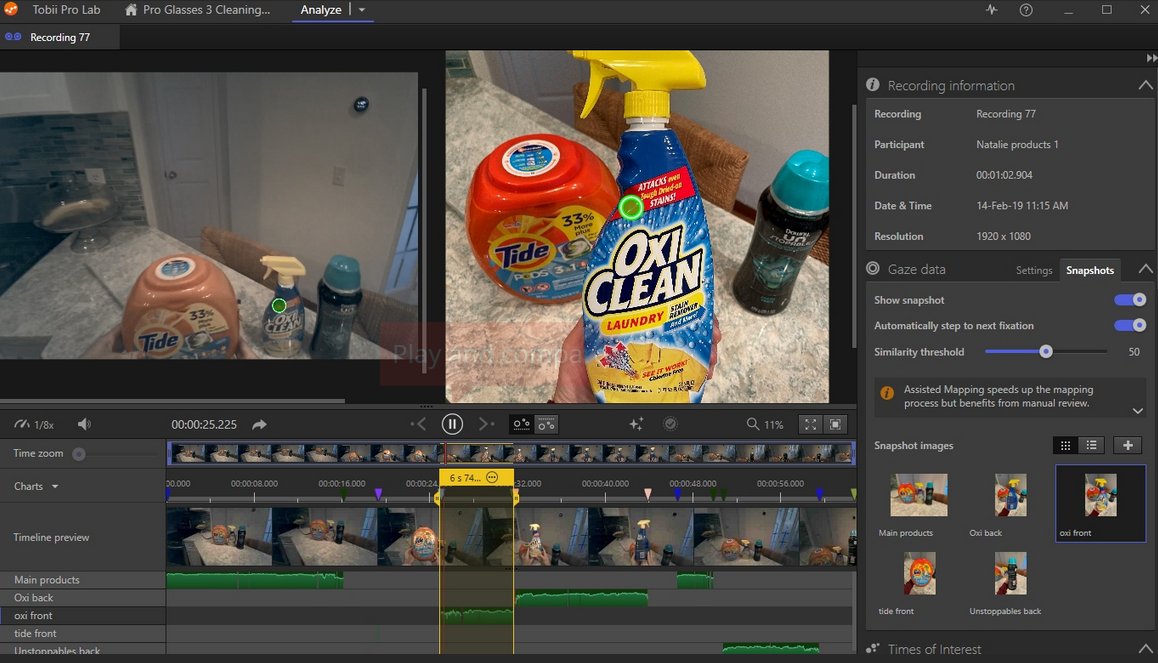
\includegraphics[width=1\textwidth]{images/04/snapshot.png}
    \caption{Ukážka s referenčným obrázkom z iného výskumu. Naľavo je video záznam a napravo je zobrazený referenčný obrázok, na ktorý sa úspešne podarilo premietnuť pohľad z kamery.}
    \label{img:lab}
\end{figure}

% tensorboard https://medium.com/mlearning-ai/remote-tensorboard-viewing-on-your-local-browser-b0dc5c5a634a     and     https://pytorch.org/docs/stable/tensorboard.html

\section{Detektor reklám}

Narozdiel od predchádzajúcich YOLO verzií sa dá YOLOv8 nainštalovať a importovať do projektu priamo ako knižnica pre Python. Spolu s ňou sa do prostredia nainštalujú ďalšie dôležité knižnice ako matplotlib, opencv-python, scipy, torch, torchvision a iné. Trénovanie sa spúšťa pomocou jedného príkazu, kde argumenty špecifikujú hodnoty pre parametre. Potrebné je nastaviť tri parametre, ostatné majú prednastavené hodnoty podľa všeobecného odporúčania pre prvý tréning.

\begin{enumerate}
    \item Zdroj dát: v našom prípade priečinok uložený na disku, ale dá sa použiť aj živý záznam z kamery alebo odkaz na video zverejnené na internete.
    \item Počiatočné váhy: dajú sa stiahnuť z oficiálnej dokumentácie pre YOLOv8. Na výber je 5 modelov, ktoré sa líšia počtom parametrov, rýchlosťou a presnosťou.
    \item Počet epoch: určuje koľko krát prejdú všetky tréningové dáta sieťou. Po každej epoche sa vyhodnotí úspešnosť na validačnej sade.
\end{enumerate}

%\begin{figure}[ht]
%    \centering
%    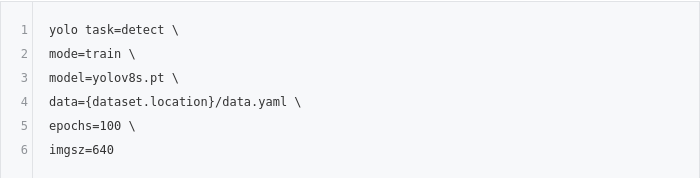
\includegraphics[width=1\textwidth]{images/04/cmd.png}
%    \caption{Ukážka .}
%    \label{img:cmd}
%\end{figure}

Po natrénovaní sa dá spustiť testovanie a detekcia zo získaných váh. V prípade testovania, musia byť na vstupe okrem obrázkov aj pravdivé označenia, podľa ktorých sa vyhodnotí úspešnosť. V prípade detekcie postačí obrázok alebo video z ktorého chceme získať detekcie. V oboch prípadoch je najdôležitejším parametrom hodnota prahu pre detekciu. Táto hodnota určuje, aká vysoká musí byť pravdepodobnosť, aby sa detekcia považovala za úspešnú. Okrem toho sa dá nastaviť očakávaný výstup. Výstup môže byť textový súbor s detekciami, ale aj obrázky s vykresleným alebo vystrihnutým označením.

\subsection{Dataset}

Väčšina obrázkov v Mapillary Vistat je vyhotovená z vnútra, prípadne zo strechy vozidla. Obrázky zachytávajú premávku vo vnútri mesta, kde sa nachádza veľa budov, chodníkov, dopravných značení a mnoho iných objektov z cestnej premávky vrátene reklamných plôch.

Anotácie sú uložené vo formáte, ktorý nie je kompatibilný s formátom pre YOLO. Počas úpravy formátu sme zároveň vynechali obrázky, ktoré neobsahovali reklamu, čím sa počet obrázkov znížil na približne 20000 obrázkov. Pri prvom tréningu sme si všimli, že veľká chybovosť nastáva práve pri najmenšie označených reklamách. Najmenšie reklamy boli označené v takej diaľke, že by sa nedalo s istotou povedať, či sa vodič skutočne pozeral na reklamu, alebo na iný objekt. Preto sme z pôvodných dát vytvorili druhú verziu, kde sme ponechali len také obrázky, kde reklamná plocha tvorí aspoň 0,1\% z obrázka. Takouto úpravou mala druhá verzia dát takmer o polovicu menej obrázkov.

Pripravili sme ešte tretiu verziu dát, kde sme k vytriedeným dátam pridali 350 nových obrázkov s anotáciami reklám. Obrázky pochádzali z videí nahratých cez eyetracker, ktoré boli mimo meranú trasu. Všetky tri verzie dát sme rozdelili na tréningovú, validačnú a testovaciu sadu, v pomere 8:1:1.

\subsection{Tréning}

Počas celého trénovania sme mali k dispozícii informácie o priebežných výsledkoch. Po každej vykonenej epoche sa vypísal výsledok z testovania na validačnej sade a čas trvania jednej epochy. Hodnoty váh sa po skončení epochy uložili do súboru na disk, takže v prípade neočakávaného prerušenia tréningu, sa dalo mohlo pokračovať od posledného miesta. Ak bol výsledok z testovania lepší ako v predchádzajúcich cykloch, tak sa hodnoty váh uložili do súboru, ktorý označoval najlepšie váhy. Pokiaľ sme si všimli, že sa vývoj tréningu nezlepšoval, mohli sme ho v hociktorom momente zastaviť. V prípade, že sme vývoj nesledoval a vývoj sa nezlepšoval, tak sa tréning po 50 epochách ukončil automaticky.

Vývoj sa dal sledovať aj vizuálne. Po každej epoche sa vykreslil graf, ktorý zobrazoval vývoj straty, presnosti a citlivosti na tréningovej a validačnej sade. Vývoj jedného tréningu je zobrazený na obrázku \ref{img:graf}. Priebeh grafu v treťom stĺpci pre test z validačnej sady ukazuje, že sa hodnota straty začala približne v 50 epoche zväčšovať. Podobný vývoj je na grafoch pre metriku recall a mAP, kým metrika precision stále mierne zvyšovala svoju hodnotu. Je to znakom preučenia, kedy sa sieť naučila rozpoznávať trénovacie dáta, ale zlyháva pri rozpoznávaní nových dát. V tomto prípade malo zmysel ukonžiť tréning predčasne.
\\
\begin{figure}[ht]
    \centering
    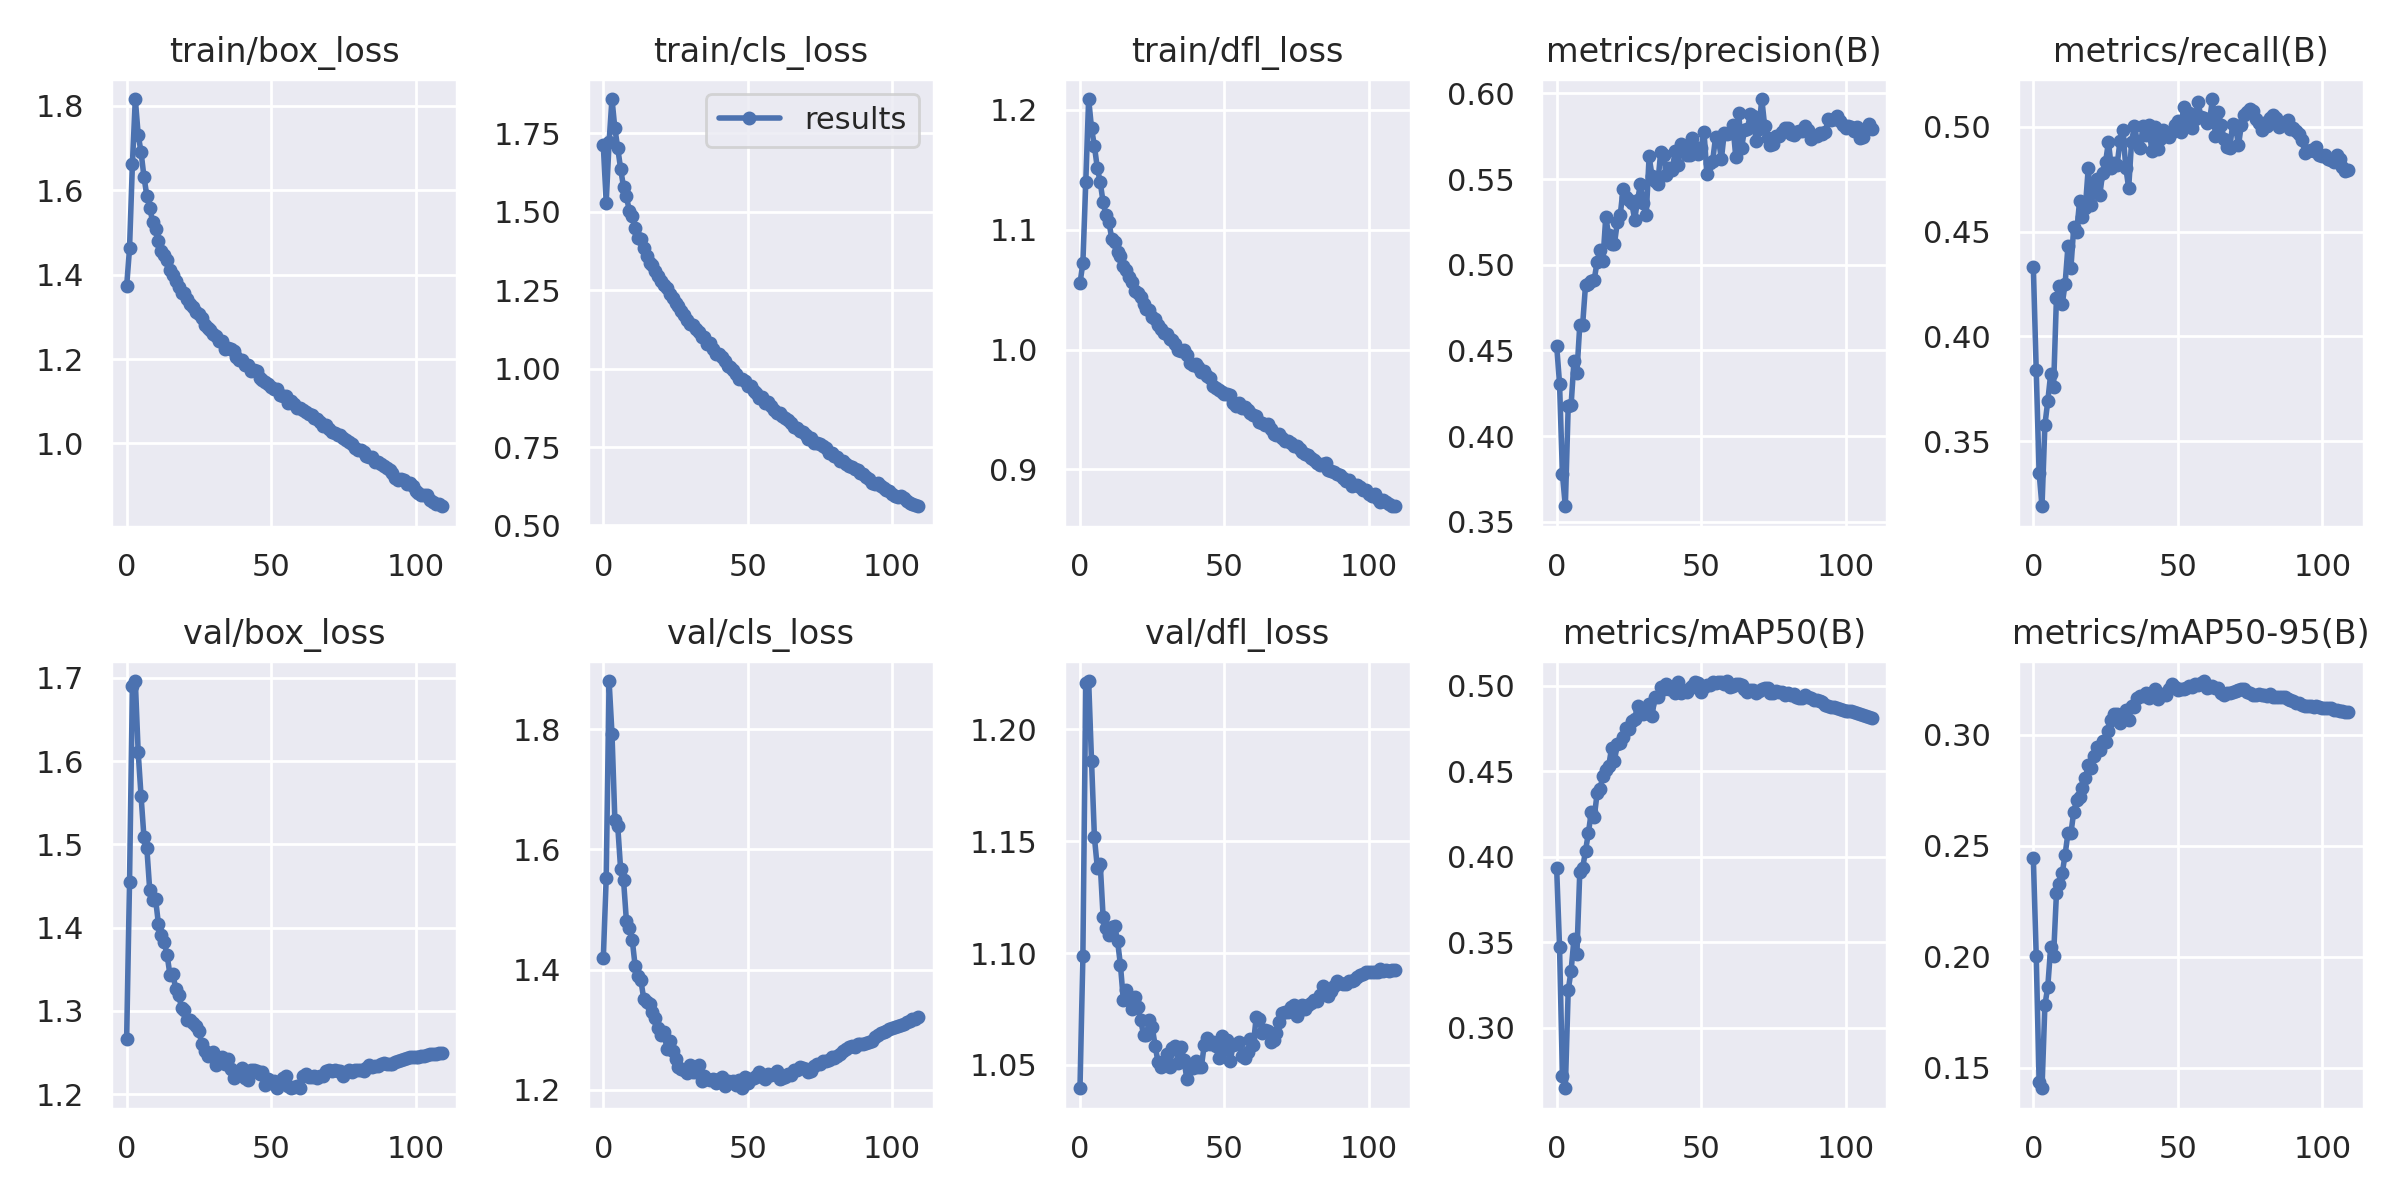
\includegraphics[width=1\textwidth]{images/04/graf.png}
    \caption{Vývoj tréningu aktualizovaný po vykonanej epoche.}
    \label{img:graf}
\end{figure}

\subsection{Sledovanie reklám}

% https://velog.io/@mink7878/Object-Tracking-Simple-Online-and-Realtime-Tracking-SORT-%EB%85%BC%EB%AC%B8-%EB%A6%AC%EB%B7%B0

Na sledovanie reklám vo videách sa nám podarilo nájsť repozitár \cite{mikel}, v ktorom je možné vyskúšať viaceré sledovacie metódy. V čase keď sme s ním pracovali, podporoval metódy OC-SORT \cite{ocsort}, Deep OC-SORT \cite{deepocsort}, StrongSORT \cite{strongsort}, BoTSORT \cite{bot} a ByteTrack \cite{bytetrack}. Všetky metódy sú implementované v jazyku Python a využívajú knižnicu PyTorch. Vychádzajú z metódy SORT (Simple Online and Realtime Tracking), ktorá na sledovanie objektov používa Kalmanov filter a Hungarian algoritmus \cite{sort}.

Vstupné video sa spracováva postupne po jednej snímke. Zo snímky sa pomocou modelu získajú detekcie, ktorým sa podľa asociácie priradí referencie. Naraz sa dajú sa sledovať viaceré objekty a triedy. Tak ako vidno na obrázku \ref{img:tracking}, výstupom sledovacej metódy sú detekcie s priradenou referenciou, ktoré vytvárajú trajektóriu sledovaného objektu.

 \begin{figure}[ht]
     \centering
     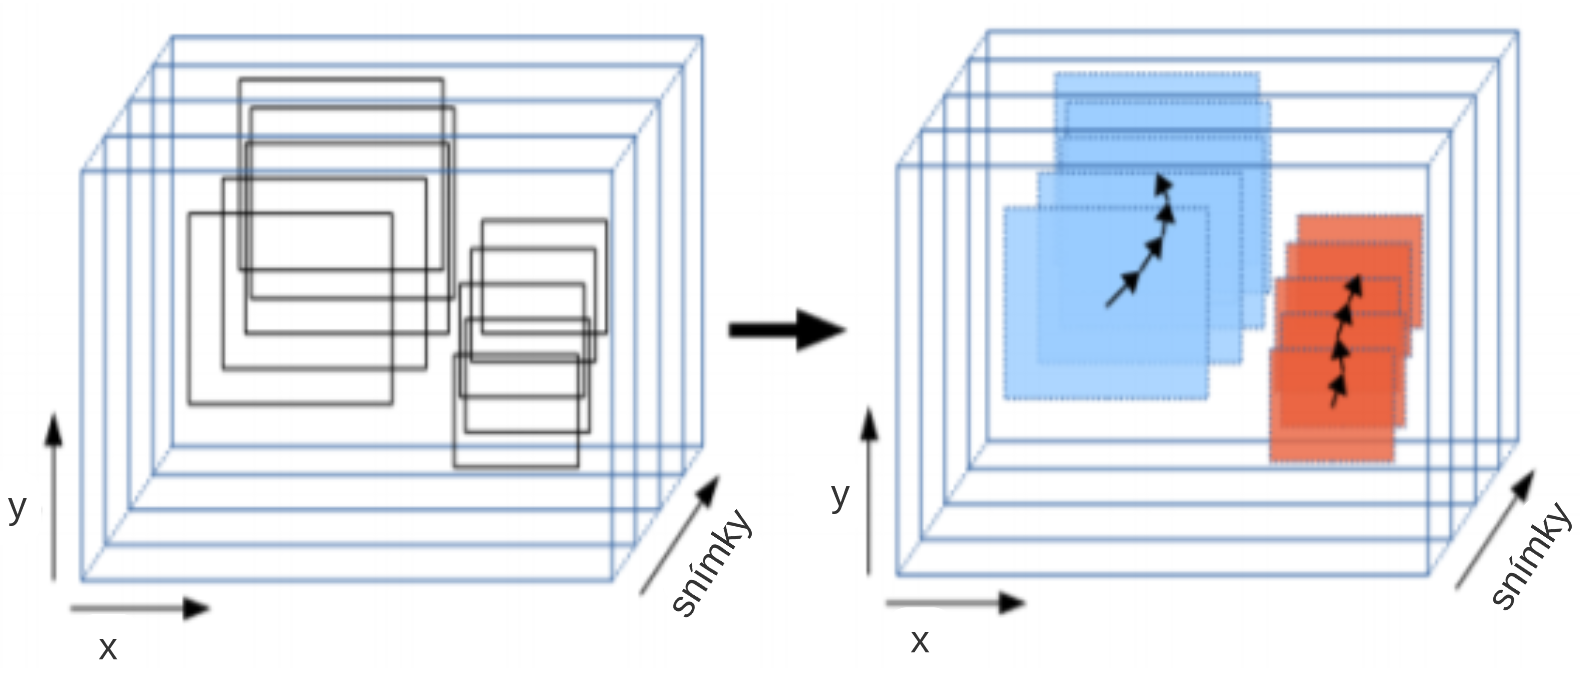
\includegraphics[width=0.7\textwidth]{images/04/tracking.png}
     \caption{Sekvencia piatich snímok, získané sú najkôr detekcie a potom referencie.}
     \label{img:tracking}
 \end{figure}

Každá metóda má vlastný konfiguračný súbor, kde sa dá nastaviť viacero parametrov, ktoré ovplyvňujú sledovanie objektu. Dva najdôležitejšie parametre sú prahová hodnota pre detekciu objektu a prahová hodnota pre asociáciu k objektom v predchádzajúcich snímkach. Okrem toho sa dá nastaviť počet predchádzajúcich snímok, v ktorých sa porovnáva asociácia objektov, minimálny počet snímok na vytvorenie novej referencie a niekoľko ďalších parametrov špecifických pre jednotlivé metódy. Napríklad pre StrongSORT je to maximálna vzdialenosť lokalizácie a pre OC-SORT výber asociačnej funkcie.

\subsubsection{Pozorovanie metód}

Na vystrihnutej časti zo záznamu sme vyskúšali všetky metódy s rôznym nastavením parametrov. V tomto momente sme výsledky vyhodnotili iba pozorovaním, pretože sme nemali skutočne pravdivé údaje o výskyte reklám. Bolo vidno, že niektoré reklamy vôbec neboli objavené a pre niektoré chýbali detekcie len v určitých snímkach. Ďalšia chybovosť bola v priraďovaní referencií. Stávalo sa, že niektorá reklama dostala po čase inú referenciu ako na mala na začiatku. Opačný prípad bol, keď reklama viac nebola viditeľná a tá istá referencia bola priradená pre novú reklamu. Odhadli sme, že najlepšie výsledky dosiahla metóda StrongSORT, pretože na výstup uložila najmenší počet referencií a najviac označení.

% DeepSORT je rozšírením pre SORT, ktorý integruje informácie o vzhľade získané z predtrénovaného modelu. Výsledkom je lepšie priradenie správnej identity čo zároveň redukuje počet vytvorených identít \cite{deepsort}. ByteTrack sa zameriava na asociáciu údajov a navrhuje novú metódu Byte, ktorá sleduje priradenie s porovnávaním každého objektu, ktorý bol doposiaľ zaznamenaný \cite{bytetrack}. OC-SORT je metóda, ktorá používa pozorovanie objektov na výpočet virtuálnej trajektórie počas prekrytia objektu, aby sa zmiernilo hromadenie chýb Kalmanovho filtra, ktoré vzniká počas oklúzie \cite{ocsort}. StrongSORT je varianta, ktorá pridáva pohybový model založený na optickom toku na zlepšenie výkonu sledovania pričom sa snaží kombinovať výhody z metódy Deep SORT a ByteTrack \cite{strongsort}. Každý model má sadu parametrov, ktoré sme jemne upravovali a sledovali zmenu vo výsledkoch. https://www.tasq.ai/blog/object-tracking/

\subsection{Pomocné dáta a model}

Na priblíženie sa ku skutočným výskytom reklám, sme sa rozhodli natrénovať nový pomocný model. Pre tento účel sme pripravili dataset, ktorý bol vytvorený zo snímok vystrihnutých z nahrávok experimentu. Reklamné plochy na vystrihnutých snímkam sme najskôr dali detegovať pomocou najlepšieho modelu, ktorý sme v tom momente mali. Získané označenia sme spolu s obrázkami pridali do webovej aplikácie Darwin v7labs \cite{v7}, kde sme následne opravili vzniknuté chyby z detekcie. Opraviť bolo treba približne každý druhý obrázok, ktorých spolu bolo takmer tisíc.

\begin{figure}[ht]
     \centering
     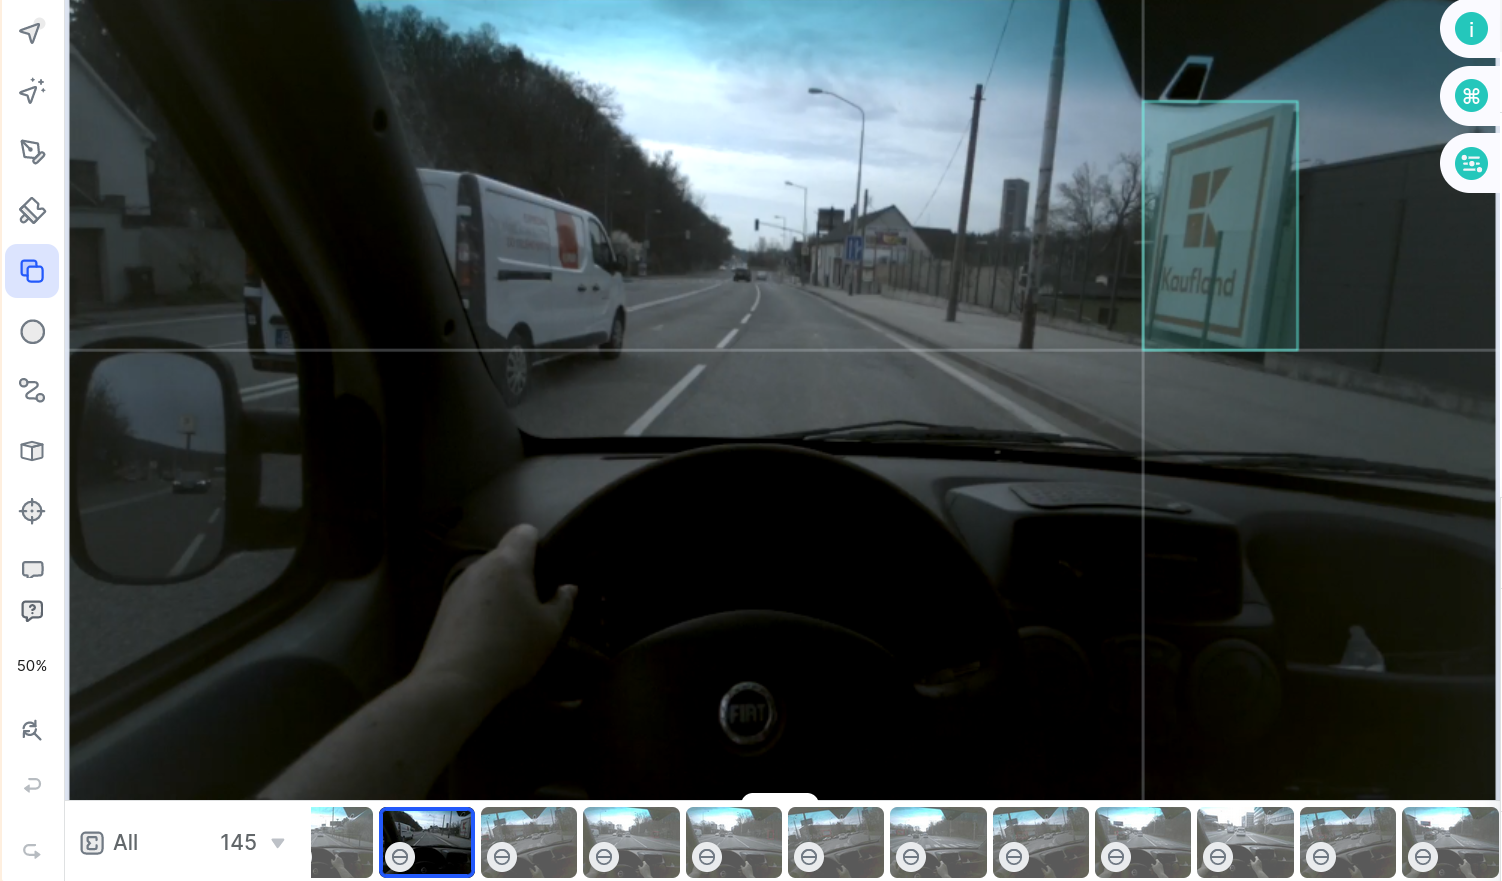
\includegraphics[width=1\textwidth]{images/04/lab.png}
     \caption{Prostredie na vytváranie anotácii vo webovej aplikácie Darwin v7labs.}
     \label{img:lab}
 \end{figure}

Pomocný model dosahoval pri sledovaní výrazne viac detekcií. Pre účely dosiahnuť čo najviac snímok s reklamou, sme metódu StrongSort nastavili tak, aby mala čo najväčšiu citlivosť detekcie. Samozrejme sa tým znížila celková presnosť sledovania, ale to v podstate nebolo dôležité, pretože sme vedeli, že pred pokračovaním budeme potrebovať každú reklamu označiť rovnakou referenciou v každom videu, aby sme mohli analyzovať pohľady na reklamu v každom videu.

Museli sme opraviť dve chyby, falošne pozitívne detekcie a nesprávne priradenie referencie. Prakticky to znamenalo, že sme vytvorili kópie nahrávok, v ktorej boli vykreslené všetky detekcie s uvedenou referenciou a sledovali označenia. Pokiaľ išlo o správnu detekciu reklamy, tak sme priradenú referenciu nahradili poradovým číslom danej reklamy, ktorá bola rovnaké pre každé video. Zmeny referencií sme zapisovali do textovho súboru. Pokiaľ išlo o falošne pozitívnu detekciu, tak sme ju jednoducho vynechali a nezapísali do súboru s opravami.

Nakoniec sme skriptom premenovali referencie podľa poradového čísla reklamy, čím sme dosiahli, že v každom videu boli reklamy označené rovnakým číslom. Získané označenia sme ďalej považovali za skutočne pravdivé údaje. Označenia sme zapísali do textového súboru vo formáte MOT \cite{mot}. pre každé video samostatne. Každá snímka, na ktorej sa nachádzala reklama bola zapísaná v samostatnom riadku s hodnotami pre poradie snímky, referenciu reklamy, x a y súradnice ľavého horného rohu a pre rozmery reklamy.

\begin{figure}[ht]
     \centering
     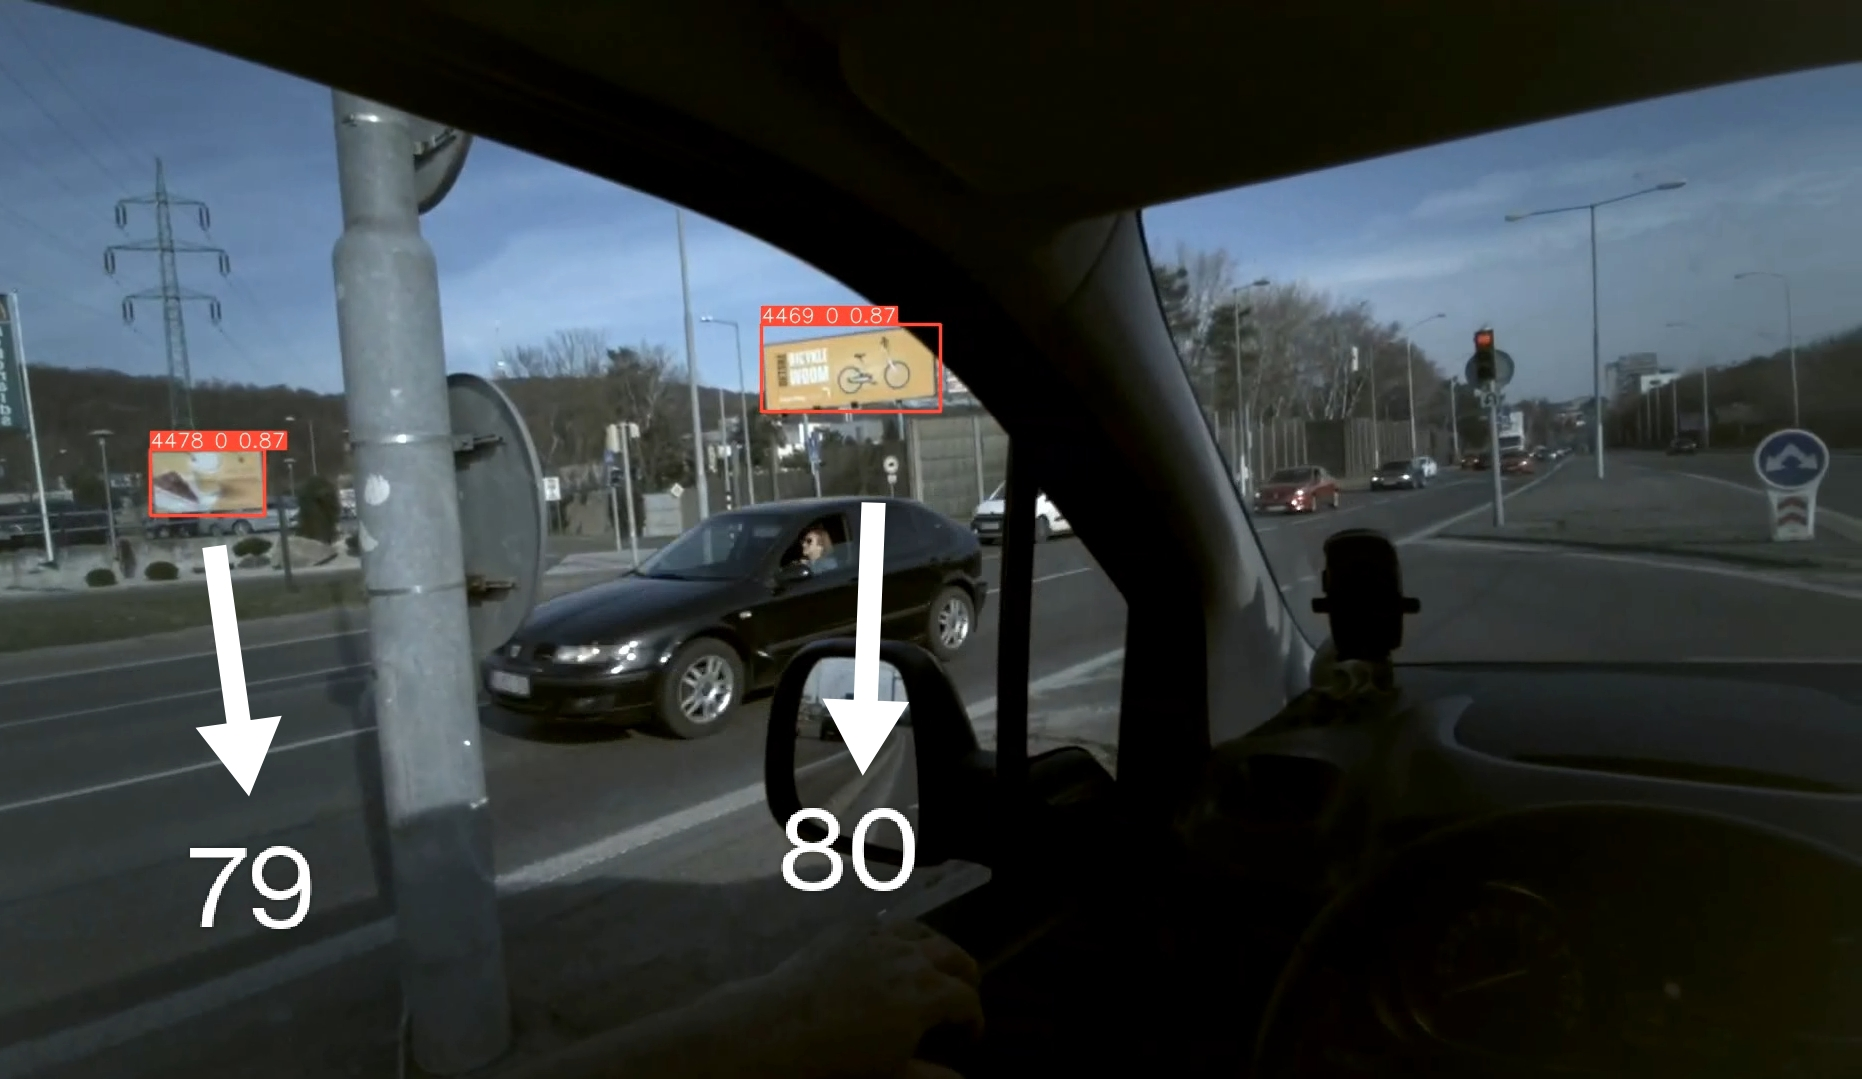
\includegraphics[width=1\textwidth]{images/04/mapping.jpg}
     \caption{Premenovanie referencií podľa poradového čísla reklamy.}
     \label{img:mapping}
 \end{figure}

\section{Významnosť reklám}

Z informácií, na ktorých snímkach sa nachádza reklama, sme mohli začať analyzovať pohľady vodičov. V tomto bode sme zistili, že pohľady boli zaznamenané v počte 50 snímok za sekundu, kým video bolo nahrávané v počte 25 snímok za sekundu. To znamená, že pokiaľ eytracker zaznamenal pohľady bez straty, tak sme mali pre každú snímku z videa dva pohľady.

Kvôli nedokonalému nahrávaniu na niektorých snímkach chýbal jeden, alebo dokonca oba pohľady. Pokiaľ sme pre snímku zaregistrovali chýbajúci pohľad, vypočítali sme jeho predikciu pomocou interpolácie dvoch predchádzajúcich pohľadov. Výpadok pohľadu na viac ako dvoch snímkach sme nepočítali a snímok sme z analýzy vynechali.

Pre každú snímku, na ktorej bola detekcia reklamy a zaznamenaný pohľad, sme porovnali prienik ich oblastí. Získali sme tým informáciu o počte snímok, kde pohľad vodiča smeroval na reklamu. Počet snímok sme vynásobili dĺžkou trvania jednej snímky, čím sme získali časový údaj sledovanosti. Podľa dĺžky sledovanosti sme vyhodnotili významnosť reklamy pre každého vodiča samostatne a následne vypočítali konečnú významnosť pomocou mediánu.

 \begin{figure}[ht]
     \centering
     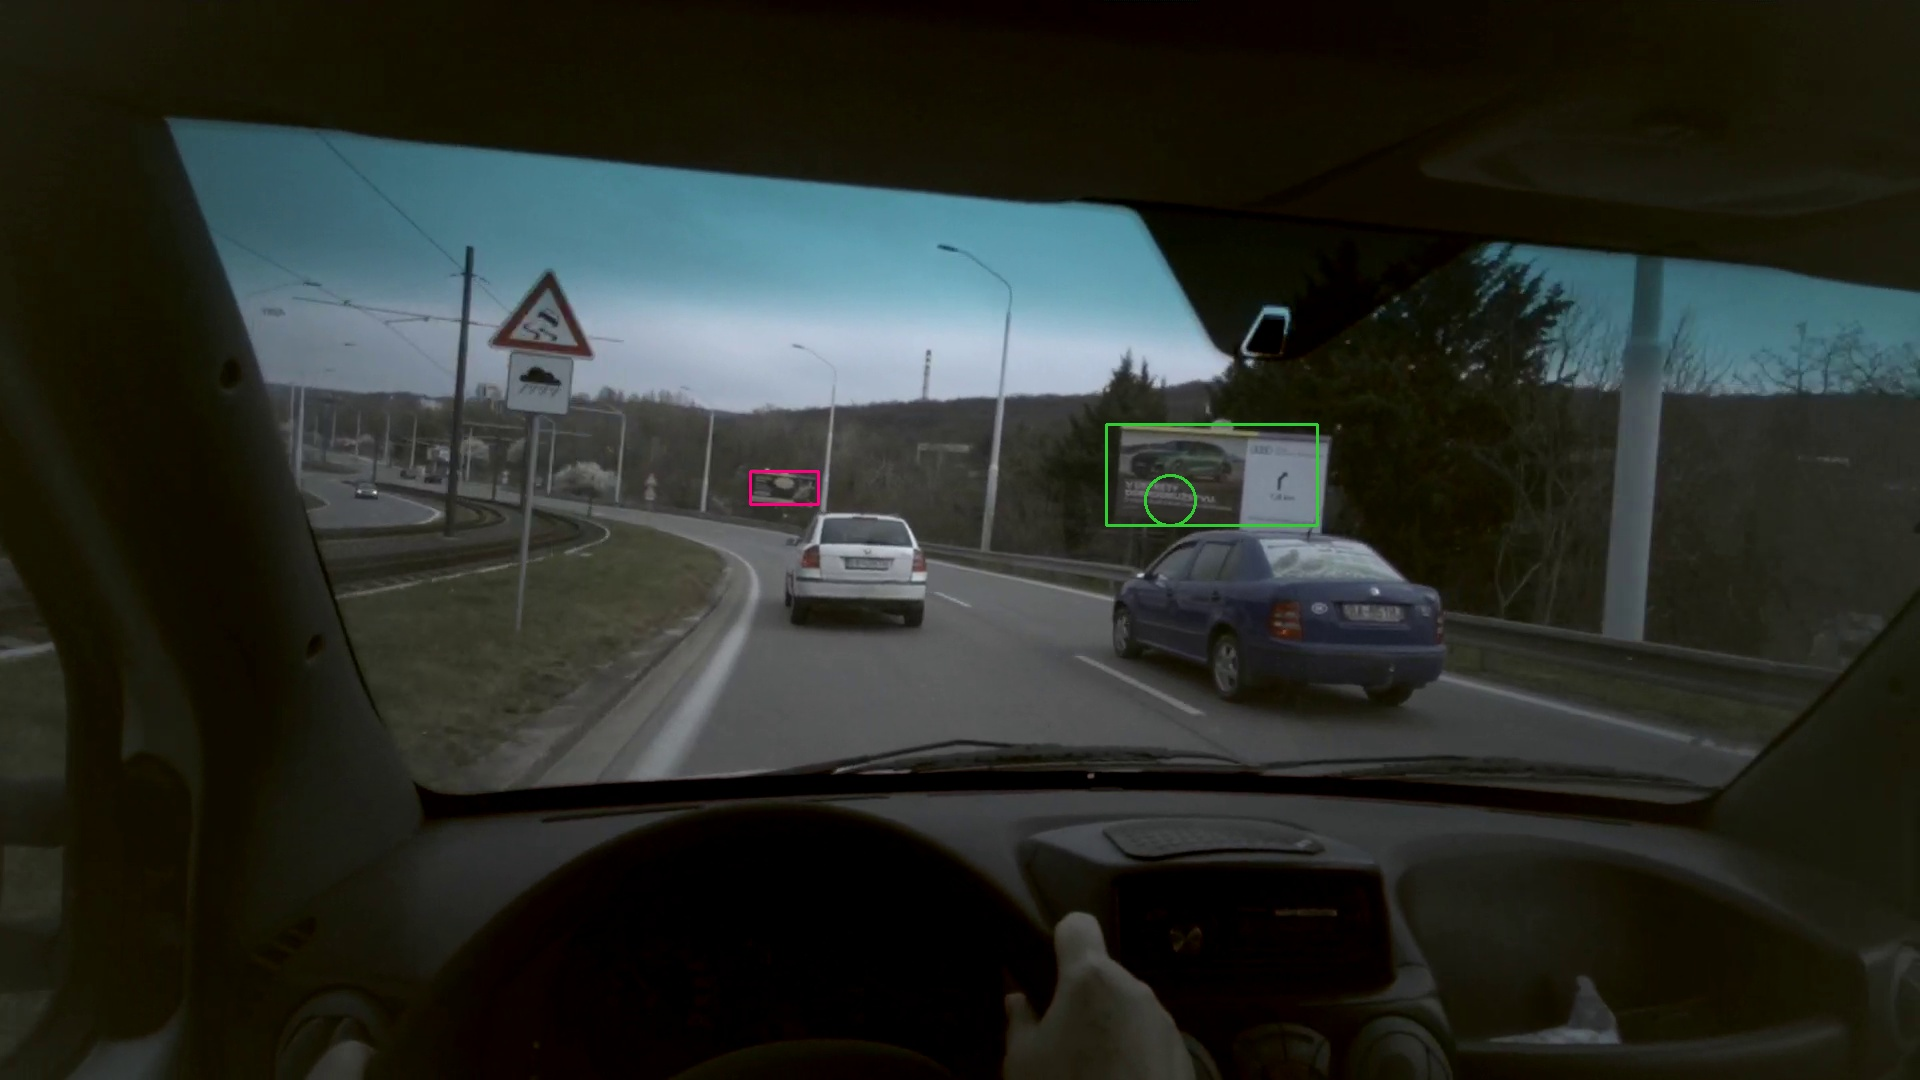
\includegraphics[width=1\textwidth]{images/04/iou.jpg}
     \caption{Na obrázku sú detekované dve reklamy, na jednej z nich sa nachádza prienik s pohľadom vodiča.}
     \label{img:tracking}
 \end{figure}

\section{Klasifikátor reklám}

S predchádzajúcimi krokmi sa nám podarilo pripraviť databázu reklám s priradenou významnosťou. Pre každú reklamu sme mali uložené všetky snímky s detekciou. Snímky boli rozdelené pre každú reklamu a pre každé video samostatne. Snímky, na ktorých sa nachádzala jedna a tá istá reklama sme nazvali sekvenciou. Pre každú sekvenciu sme vypočítali vlastnosti, ktoré sme použili na klasifikáciu.

Na to aby sme vedeli predikovať významnosť reklamy, sme natrénovali Random Forest Classifier (RFC). Podobne ako pri trénovaní neurónovej siete sme databázu rozdelili na dve časti v pomere 8:2. Tentokrát sme nepotrebovali validačnú sadu. V tréningovej sade sa nachádzalo 115 reklám a v testovacej 30.

RFC na základe hodnôt vlastností v tréningovej sade náhodne vygeneruje viacero rozhodovacích stromov. Rozhodovací strom je tvorený z vrcholov, v ktorých sa nachádza podmienka, podľa ktorej sa zo vstupných údajov vytvorí cesta ku listu. Podmienka porovnáva hodnotu danej vlastnosti s navrhnutou prahovou hodnotou. Na konci vetvy je v liste uložená trieda, ktorá určuje významnosť reklamy.

Pri testovaní sa významnosť reklamy predikuje tak, že sa vstupné údaje (vektor príznakov) vložia do rozhodovacieho stromu a podľa podmienok sa vypočíta hodnota významnosti. Významnosť reklamy je určená hodnotou triedy, ktorá sa vyskytovala najčastejšie zo všetkých rozhodovacích stromov.
% todo nahradiť slovo vlasnosť za slovo príznak; skupina príznakov sa nazýva vektor príznakov

\subsection{Extrahovanie príznakov}

Každý reklama mala nanajvýš 8 sekvencíí. V niektorých videách nebol detekovaný úplný počet reklám, kvôli tomu že reklamu mohlo zakrývať auto alebo bola v takom uhle, že keď bol vodič vo vzdialenejšom jazdnom pruhu, tak ju nebolo vidno. Hodnota vlastnosti bola vypočítaná ako priemerná hodnota zo všetkých sekvencií reklamy.

\subsubsection{Počet snímok v sekvencii}

Najjednoduchšia vlastnosť je počet snímok, ktoré sa nachádzajú v sekvencii. Táto vlastnosť nám hovorí o tom, ako dlho bola reklama viditeľná. Čím dlhšie bola reklama viditeľná, tým väčšiu mala šancu, že ju vodič zaregistruje.

\subsubsection{Lokalizácia reklamy}

Z lokalizácie reklamy sme vypocítali dva príznaky. Prvý príznak určoval, na ktorej strane obrazu sa reklama nachádzala najdlhšie. Obraz sme rozdelili na ľavú, právu a strednú časť. Stredná časť bola definovaná v rozmedzí 20\% od stredového bodu, ľavá a práva časť zaberala po 40\% plochy.

Vodiči majú tendenciu pozerať sa do stredu obrazu, preto reklamy, ktoré sa nachádzali v strede obrazu, mali väčšiu šancu, že ich vodič zaregistruje. Na základe toho sme vypočítali druhý príznak, ktorý určoval euklidovskú vzdialenosť stredného bodu reklamy od stredu bodu obrazu.

\subsubsection{Veľkosť reklamy}

Veľkosť sme vypočítali ako pomer reklamnej plochy a plochy snímky. Ak bola reklama detekovaná vo väčšej vzdialenosti, tak jej priemerná veľkosť bola menšia než v prípade reklamy detekovanej v bližšej vzdialenosti aj napriek rovnakému rozmeru. Vozidlo sa k reklame približovalo, preto sme okrem priemernej veľkosti z celej sekvencie vypočítali aj priemernú veľkosť v posledných desiatich snímkach.

\subsubsection{Mapa význačností}

Na výpočet sme použili existujúcu neurónovu sieť HD2S \cite{hd2s}, určenú na získavanie máp význačností z videí. V tom čase mala najlepšie výsledky na viacerých testovacích databázach, ak nepočítame sieť ViNet \cite{jain2021vinet}, z ktorej sa nám nepodarilo získať žiadny výstup.

Každú video nahrávku sme vložili celú na vstup a neurónová sieť nám vrátila mapu význačností pre každú snímku. Podobne ako v predchádzajúcich prípadoch, sme vypočítali hodnotu príznaku pre každú sekvenciu samostatne. V tomto prípade nás zaujímali dve veci. Priemerná hodnota význačnosti v celej snímke a priemerná hodnota význačnosti v oblasti ohraničenia reklamy.

Veľká časť snímky mala nulové, prípadne iné nízke hodnoty, ktoré výrazne znižovali priemer. Preto sme priemer počítali len z významnejších oblastiach. Prahovú hodnotu sme nastavili na X. Nakoniec sme pre každú sekvenciu uložili ešte tretí príznak, ktorý bol pomer medzi priemernou hodnotou význačnosti v oblasti ohraničenia reklamy a priemernou hodnotou význačnosti v celej snímke.

TODO prečo.

\subsubsection{Entropia reklamy}

TODO prečo.

TODO ako.

TODO kód.